\begin{frame}{Análisis de los resultados obtenidos I}
	\begin{itemize}
		\item \textbf{Tamaño de batch}\arrowTikz{0}32
		\item \textbf{Número de FFT}
		\begin{itemize}
			\scriptsize
			\item Entrenamiento\arrowTikz{0}63132
			\item Validación\arrowTikz{0}4068
		\end{itemize}
		\item \textbf{Número de épocas}\arrowTikz{0}2000\footnote{\scriptsize El entrenamiento se paró en 1390 al comprobar que los resultados empeoraban}
		\item \textbf{Tasa de aprendizaje}\arrowTikz{0}Decreciente en el tiempo.
	\end{itemize}
	\begin{figure}
		\centering
		\begin{subfigure}[t]{0.45\textwidth}
			\centering
			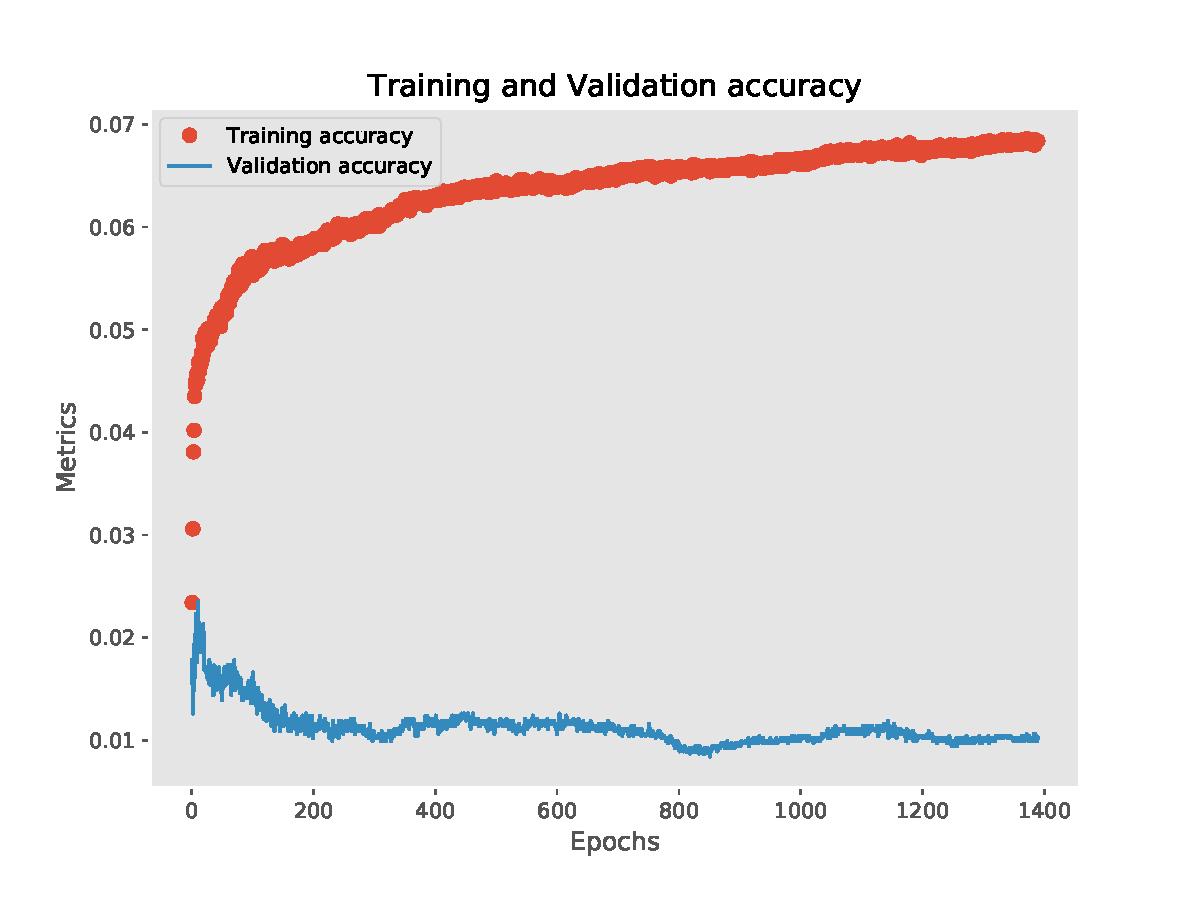
\includegraphics[width=\textwidth]{../figures/one_to_one_results_acc.pdf}
			\vspace*{-7pt}
			\caption{Precisión en entrenamiento y validación}
		\end{subfigure}%
		\hspace*{10pt}
		\begin{subfigure}[t]{0.45\textwidth}
			\centering
			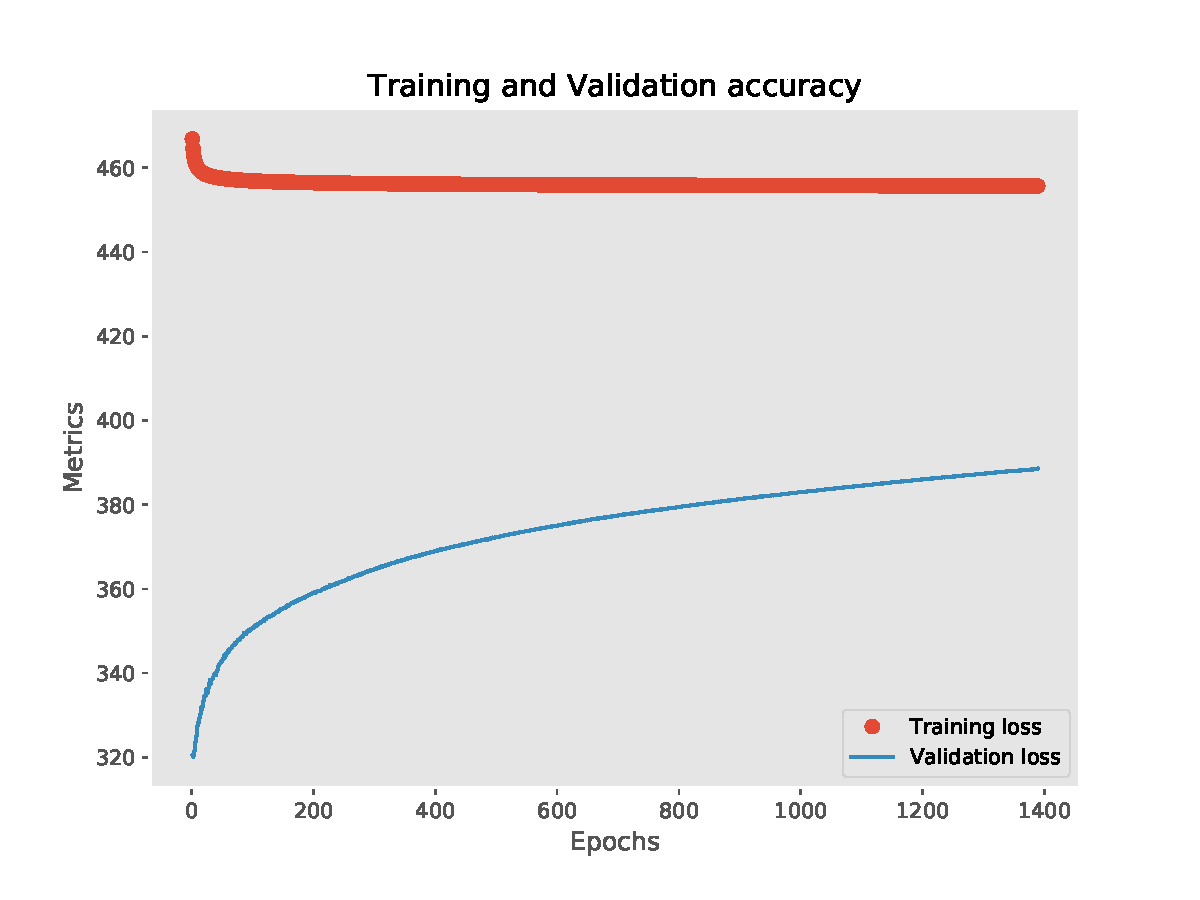
\includegraphics[width=\textwidth]{../figures/one_to_one_results_loss.pdf}
			\vspace*{-7pt}
			\caption{Pérdidas en entrenamiento y validación}
		\end{subfigure}
	\end{figure}
\end{frame}
\begin{frame}[fragile]{Análisis de los resultados obtenidos II}
\begin{lstlisting}[basicstyle=\tiny\ttfamily, caption={Resumen del modelo mono-capa},captionpos=b, label={lst: model_resume_monolayer},frame=none, xleftmargin=.2\textwidth, xrightmargin=.2\textwidth]
_________________________________________________________________
Layer (type)                 Output Shape              Param #   
=================================================================
lstm (LSTM)                  (None, 2048)              18833408  
_________________________________________________________________
dense (Dense)                (None, 250)               512250    
=================================================================
Total params: 19,345,658
Trainable params: 19,345,658
Non-trainable params: 0
_________________________________________________________________
\end{lstlisting}
\begin{columns}
	\begin{column}{0.5\textwidth}
		\begin{itemize}
			\item \textbf{Tamaño de batch}\arrowTikz{0}128
			\item \textbf{Número de FFT}
			\begin{itemize}
				\scriptsize
				\item Entrenamiento\arrowTikz{0}55657
				\item Validación\arrowTikz{0}11543
			\end{itemize}
			\item \textbf{Número de épocas}\arrowTikz{0}300\
			\item \textbf{Tasa de aprendizaje}\arrowTikz{0}Decreciente en el tiempo.
		\end{itemize}
	\end{column}
	\begin{column}[t]{0.5\textwidth}
		\vspace*{-50pt}
		\begin{figure}[t!]
			\centering
			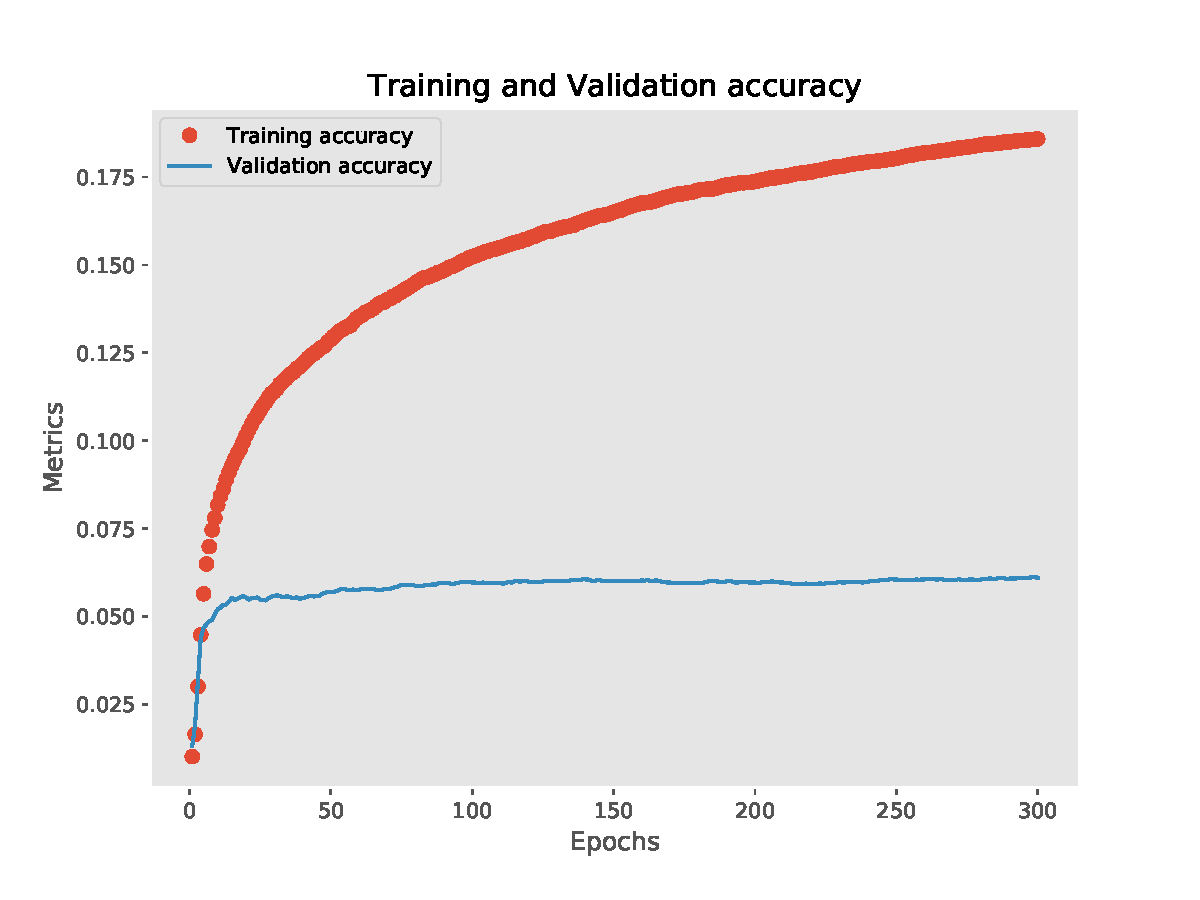
\includegraphics[width=0.9\columnwidth]{../figures/results_acc_compa.pdf}
			\vspace*{-10pt}
			\caption{Precisión en entrenamiento y validación}
			\label{fig: results_acc_compa}
		\end{figure}
	\end{column}
\end{columns}
\end{frame}